\section{Experiments}\label{sec:experiments}
This section describes the experiments that were performed and their results. All statistical analysis has been performed using R \cite{rstats}, a software environment for statistical computing.

\subsection{Experiment set-up}\label{sec:setup}
All experiments are performed in a virtual warehouse. Refer to figure \ref{fig:thewarehouse} for a visual representation of that warehouse. As can be seen, there are twenty columns and eight rows. Each row and each column are labelled with their corresponding coordinate. The bottom row represents the outside where inbound parcels arrive and where outbound parcels must be delivered to. It is assumed that the space between columns is occupied by shelves and that there is a left side to each shelf and a right side. A parcel can have a specific position on the left or right side of a shelf as destination. Therefore, all points in row 4 up to row 20 can have an outbound parcel waiting for pick-up or be the destination of an inbound parcel. At all times, the warehouse is populated by 20 agents. At any time, a parcel may enter the model, either as an outbound parcel that must be delivered to the outside or an inbound parcel that must be placed on a shelf.

\begin{figure}[H]
    \centering
    \includegraphics[width=0.9\textwidth]{thewarehouse.png}
    \caption{The warehouse in which the experiments are set}
    \label{fig:thewarehouse}
\end{figure}

\subsection{Other variables}\label{sec:othervars}
There are some variables that may have an impact on experiment results but which are not directly related to the domain of discourse, i.e. configuration of the gradient field. These are the following:

\begin{itemize}
    \item Number of agents: there are always 20 agents
    \item Size of the warehouse: 8 rows by 20 columns, with roles assigned to the different rows as specified in section \ref{sec:setup}
    \item Stop condition of the experiment: all experiments stop when 100 parcels have been delivered to their destination
    \item Parcel generation rate: The experiment starts with no parcels present in the warehouse. Each time a parcel is generated, an integer representing milliseconds from the interval $[15,000 ; 45,000]$, is generated, with equal probability for each value in that interval. This value is added to the current time of the simulator and represents the next time point when a parcel should be generated.
    \item Random number generators: The software component that generates agents and the software component that schedules parcels have their own random number generator.
    \item The seed for all random number generators used in the simulation is 123.
    \item Base strength of the agents' repulsive field: set to 0.25 units.
    \item Base strength of the parcels' attractive field: set to 1 unit.
    \item Threshold for the time-out counter in the protocol of section \ref{sec:agentarch}: set to 0 milliseconds, which effectively means there is no concept of time-outs.
\end{itemize}

\subsection{Performed experiments}
There are several types of models available to run experiments with:
\begin{enumerate}
    \item Models where the field strength of both agents and parcels does not change for the duration of the experiment (excepting parcels that leave the simulation when they are delivered and will therefore no longer influence the gradient field). The reference model is an instantiation of this type with the base strength of agents and the base strength of parcels listed in section \ref{sec:othervars}.
    \item Models where the field strength of either agents or parcels follow a linear relationship: $\emph{base-strength} + \emph{parcel-waiting-time} \times \frac{1}{\emph{time-factor}}$. If it is the field strength of the agents that is variable in this manner, this linear relationship is only valid if they're carrying a parcel (falling back on the base strength if not). If it is the field strength of the parcels that is variable, the linear relationship is only valid if they have not yet been picked up (parcels do not emit an attractive field if they have already been picked up). A model of this type will hereafter be referred to as a model of type 2.
    \item Models where the field strength of the agents increases from the base strength to a higher value when they are carrying a parcel and the parcel waiting time has reached a certain threshold value. A model of this type will hereafter be referred to as a model of type 3.
    \item Models where the field strength of the parcels increases from the base strength to a higher value if they have not yet been picked up and the parcel waiting time has reached a certain threshold value. A model of this type will hereafter be referred to as a model of type 4.
\end{enumerate}
The term ``parcel waiting time'' was defined in section \ref{sec:objectives}.

A total of 13 simulator runs have been performed:
\begin{enumerate}
    \item Run of the reference model where the field strength of both agents and parcels remains the same during the whole experiment.
    \item Run of a model of type 2 where the field strength of the agents follows the linear relationship with a \emph{time-factor} of 15,000 milliseconds.
    \item Run of a model of type 2 where the field strength of the agents follows the linear relationship with a \emph{time-factor} of 60,000 milliseconds.
    \item Run of a model of type 2 where the field strength of the agents follows the linear relationship with a \emph{time-factor} of 120,000 milliseconds.
    \item Run of a model of type 2 where the field strength of the parcels follows the linear relationship with a \emph{time-factor} of 15,000 milliseconds.
    \item Run of a model of type 2 where the field strength of the parcels follows the linear relationship with a \emph{time-factor} of 60,000 milliseconds.
    \item Run of a model of type 2 where the field strength of the parcels follows the linear relationship with a \emph{time-factor} of 120,000 milliseconds.
    \item Run of a model of type 3 where the field strength of the agents increases from the base strength to a value of 1.25 units when carrying a parcel that has reached a parcel waiting time of 15,000 milliseconds.
    \item Run of a model of type 3 where the field strength of the agents increases from the base strength to a value of 1.25 units when carrying a parcel that has reached a parcel waiting time of 60,000 milliseconds.
    \item Run of a model of type 3 where the field strength of the agents increases from the base strength to a value of 1.25 units when carrying a parcel that has reached a parcel waiting time of 120,000 milliseconds.
    \item Run of a model of type 4 where the field strength of the parcels increases from the base strength to a value of 5 units when they have not yet been picked up and the parcel waiting time has reached 15,000 milliseconds
    \item Run of a model of type 4 where the field strength of the parcels increases from the base strength to a value of 5 units when they have not yet been picked up and the parcel waiting time has reached 60,000 milliseconds
    \item Run of a model of type 4 where the field strength of the parcels increases from the base strength to a value of 5 units when they have not yet been picked up and the parcel waiting time has reached 120,000 milliseconds
\end{enumerate}

For each experiment, we have recorded the following variables for each parcel:

\begin{itemize}
    \item The parcel delivery time (this term was introduced in section \ref{sec:objectives})
    \item The time it took from arrival to the model until being picked up by an agent: the ``pick-up time''
    \item The time it took from being picked up by an agent until delivery to the parcel's destination: the ``time on route''
\end{itemize}

Note that the parcel delivery time is equal to the sum of the pick-up time and the time on route

\subsubsection{Density plots for each model}
In the following figures, the left graph depicts the density plot for the parcel delivery time, the middle graph depicts the density plot for the pick-up time and the right graph depicts density plot for the time on route.

\begin{figure}[H]
    \centering
    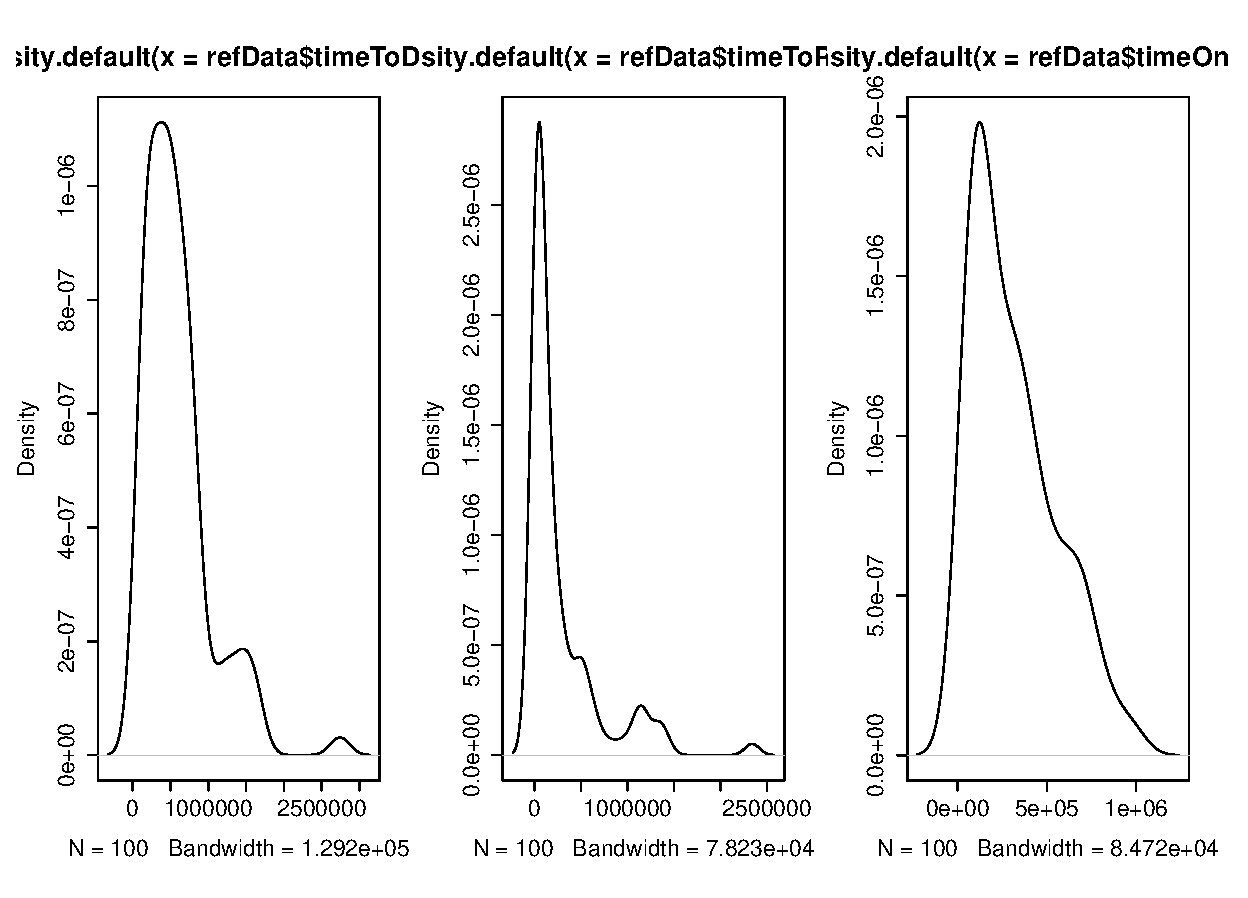
\includegraphics[width=0.7\textwidth]{densityref}
    \caption{Density plots for run 1}
    \label{fig:densityref}
\end{figure}

\begin{figure}[H]
    \centering
    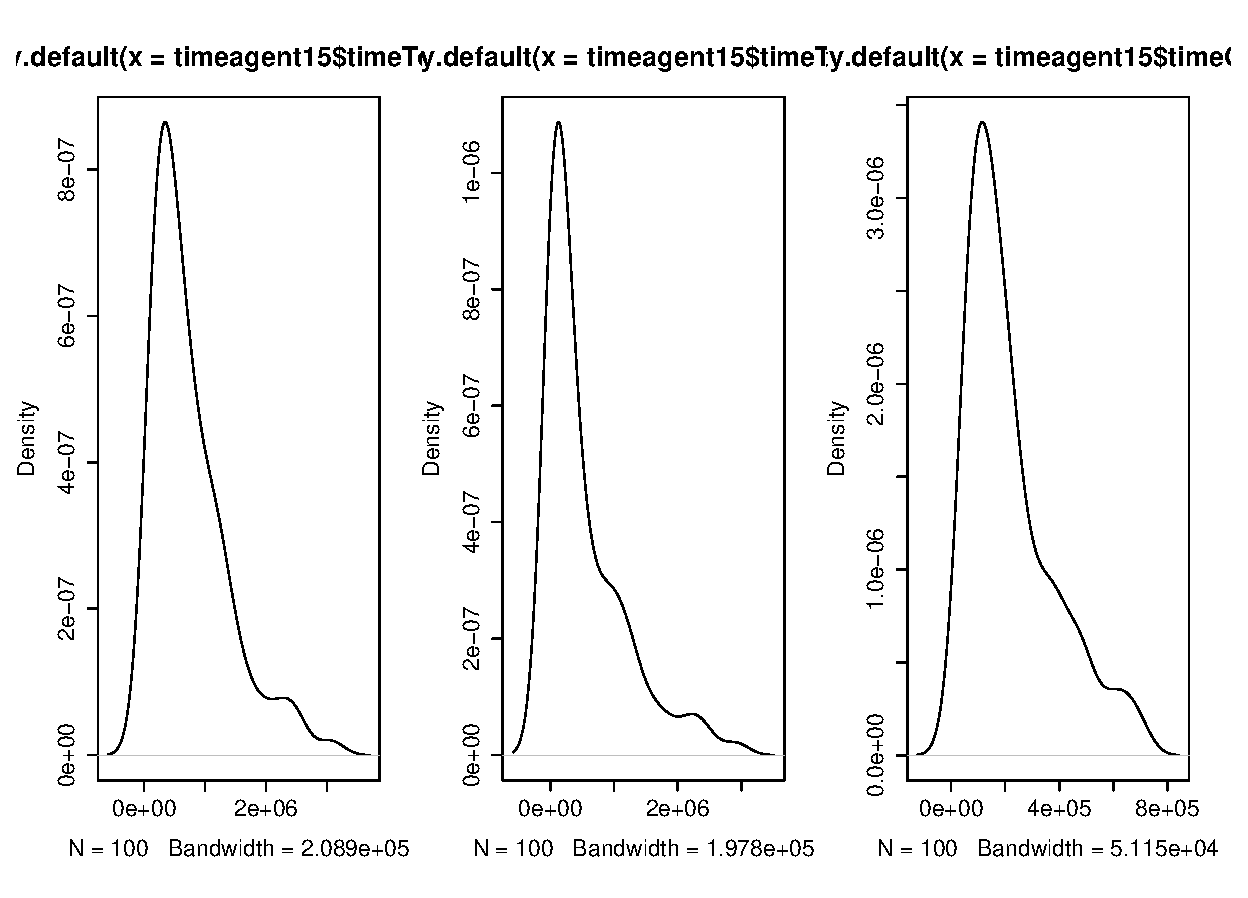
\includegraphics[width=0.7\textwidth]{densitytimeagent15}
    \caption{Density plots for run 2}
    \label{fig:densitytimeagent15}
\end{figure}

\begin{figure}[H]
    \centering
    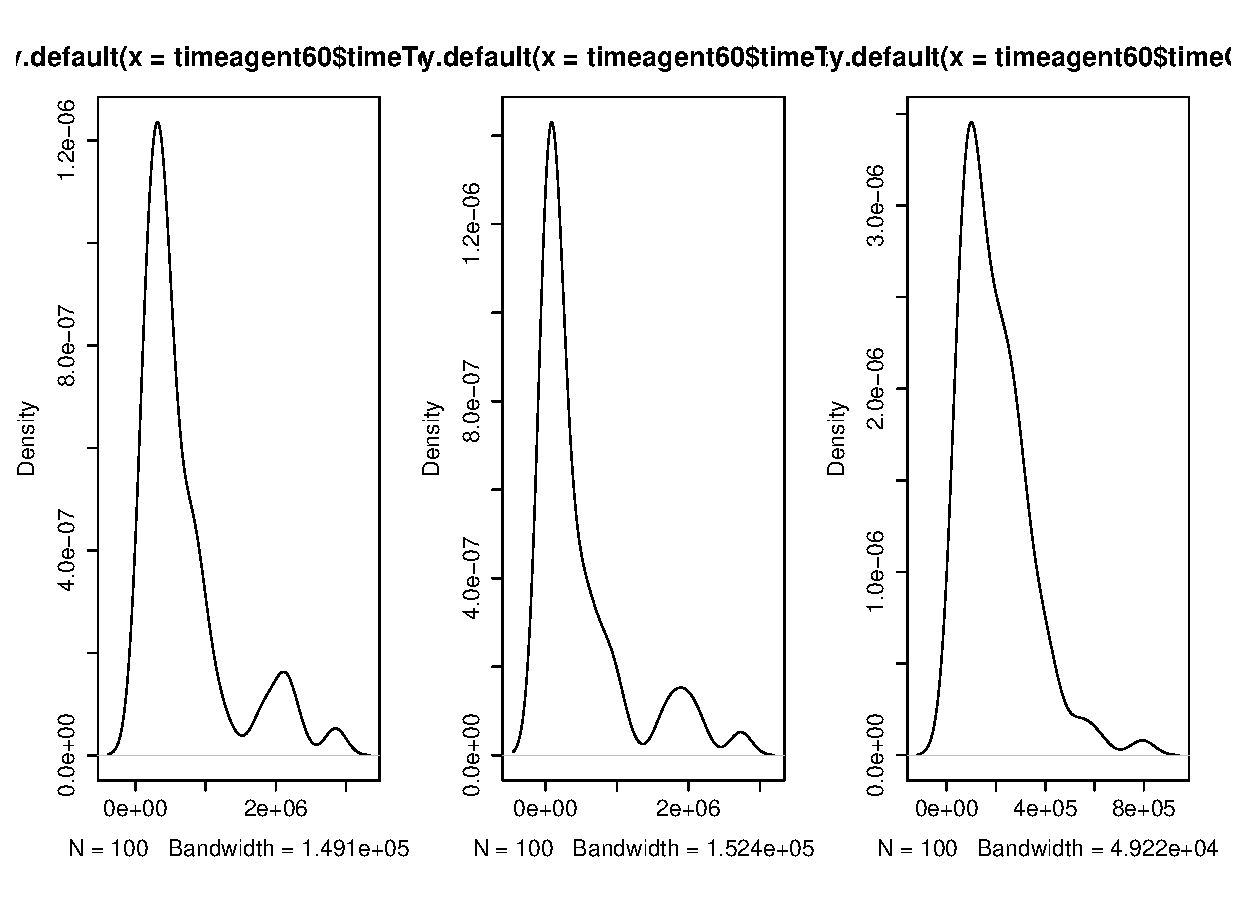
\includegraphics[width=0.7\textwidth]{densitytimeagent60}
    \caption{Density plots for run 3}
    \label{fig:densitytimeagent60}
\end{figure}

\begin{figure}[H]
    \centering
    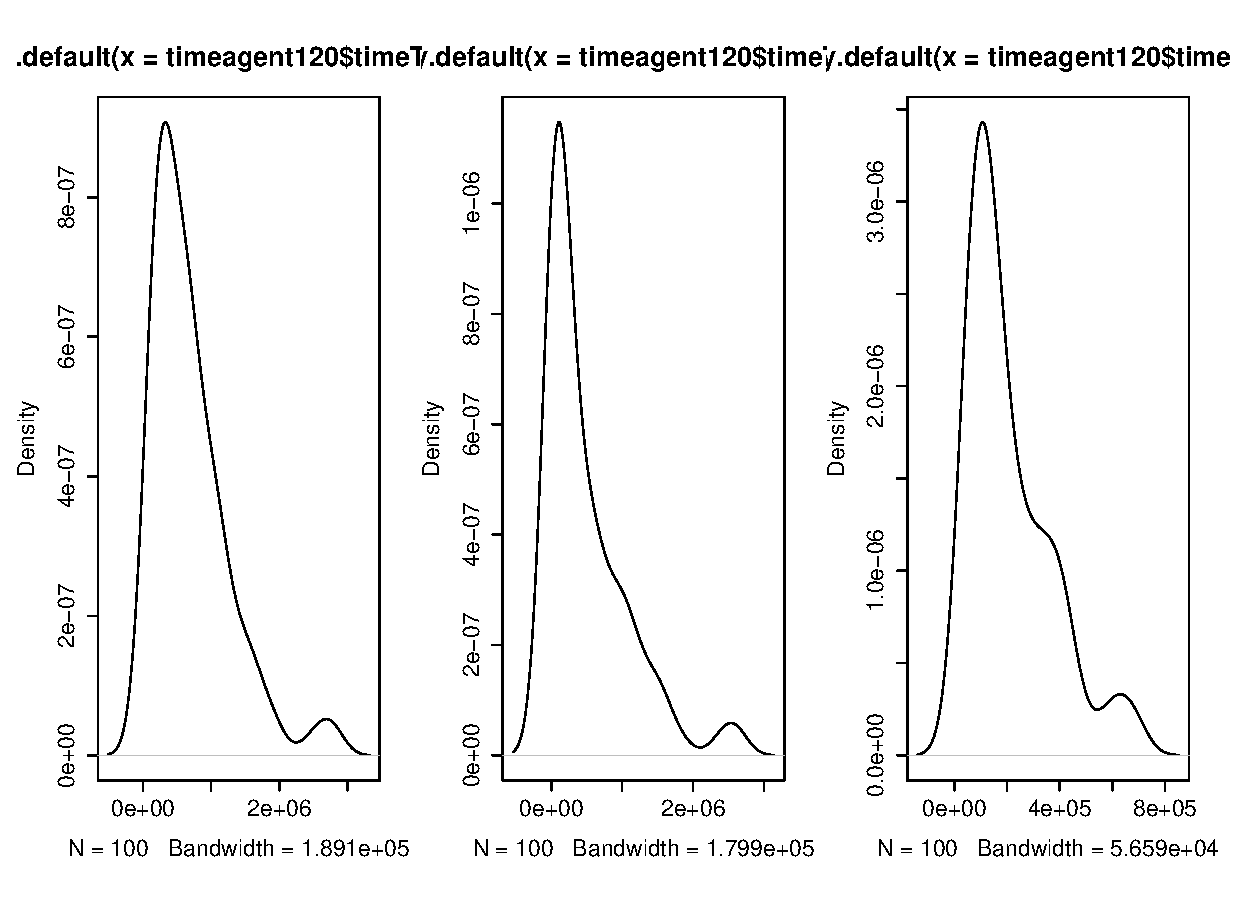
\includegraphics[width=0.7\textwidth]{densitytimeagent120}
    \caption{Density plots for run 4}
    \label{dfig:densitytimeagent120}
\end{figure}

\begin{figure}[H]
    \centering
    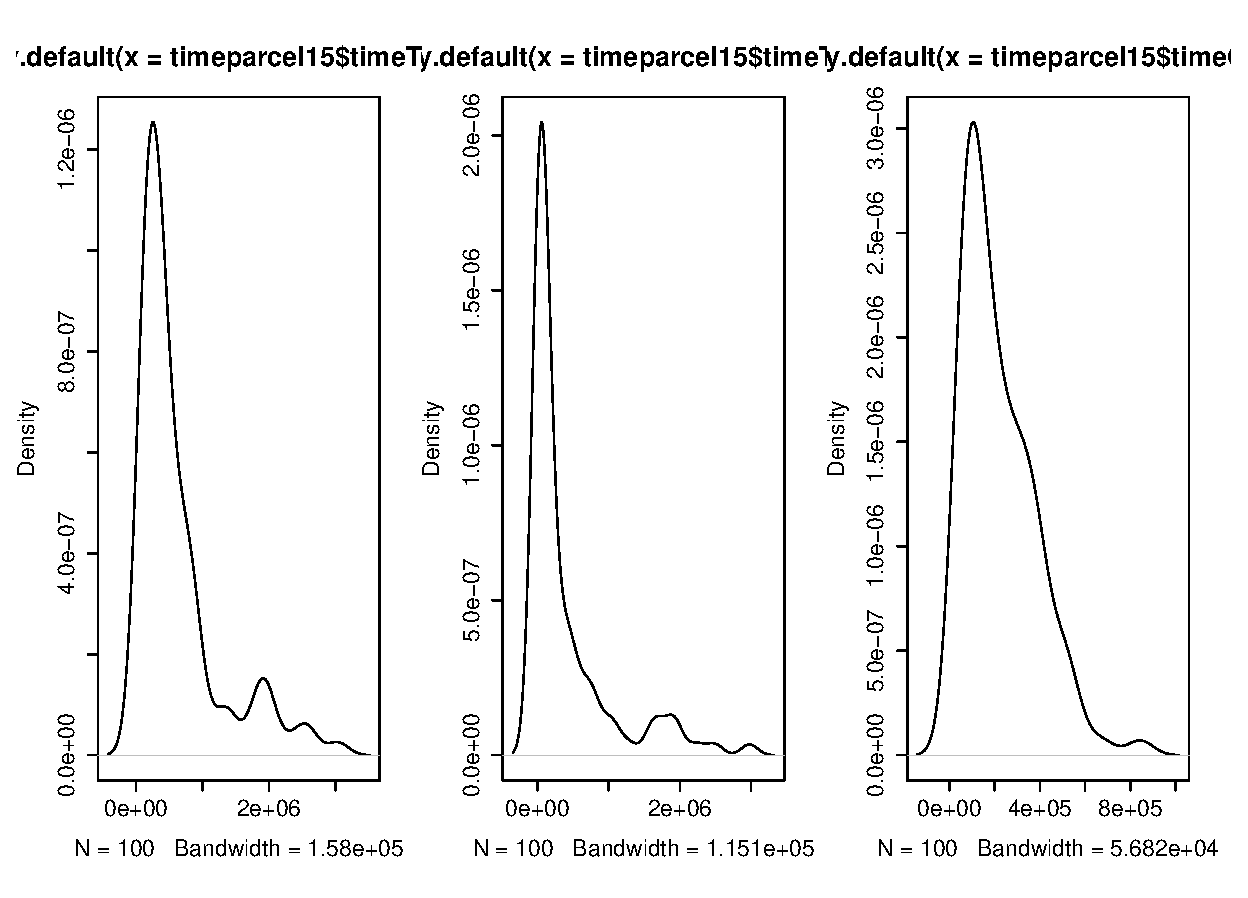
\includegraphics[width=0.7\textwidth]{densitytimeparcel15}
    \caption{Density plots for run 5}
    \label{fig:densitytimeparcel15}
\end{figure}

\begin{figure}[H]
    \centering
    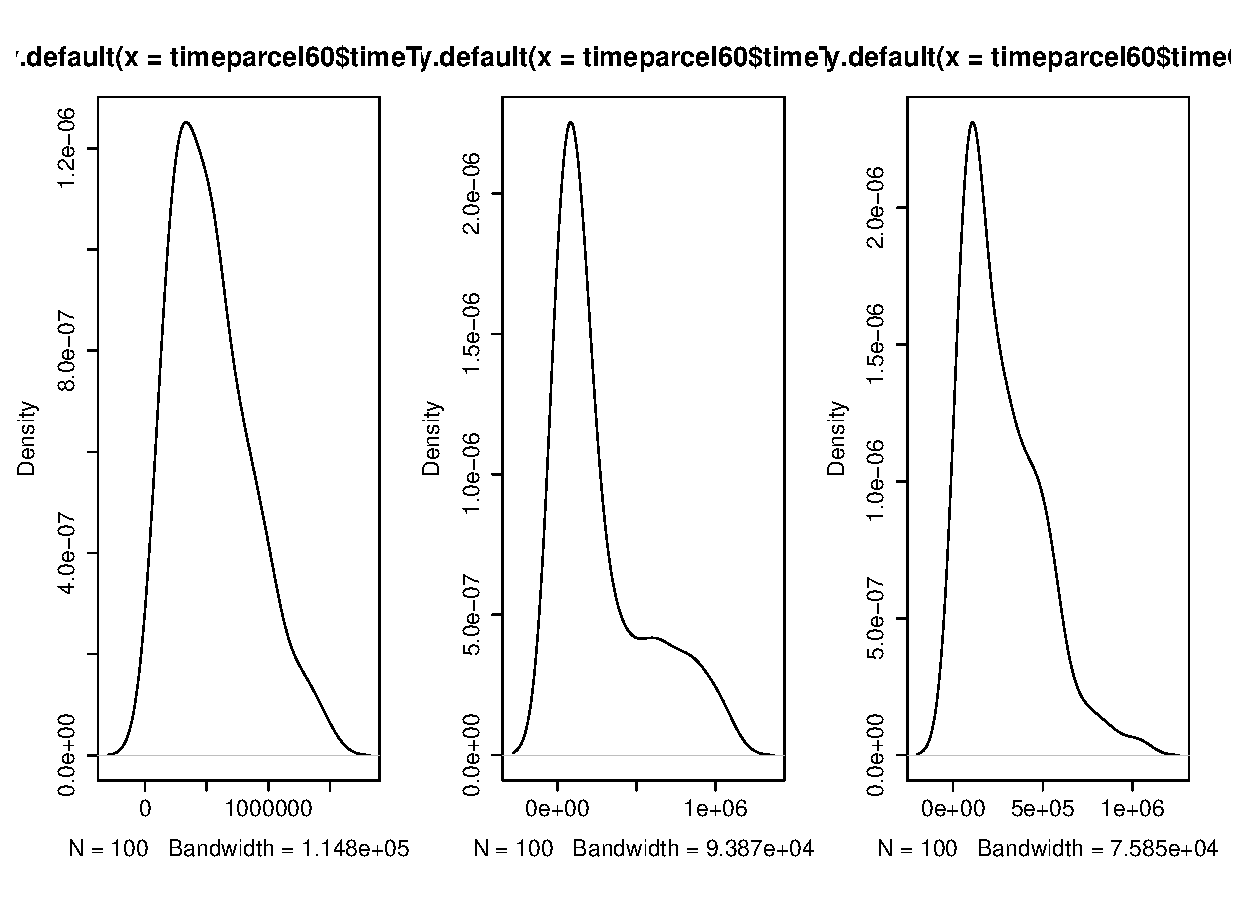
\includegraphics[width=0.7\textwidth]{densitytimeparcel60}
    \caption{Density plots for run 6}
    \label{fig:densitytimeparcel60}
\end{figure}

\begin{figure}[H]
    \centering
    \includegraphics[width=0.7\textwidth]{densitytimeparcel120}
    \caption{Density plots for run 7}
    \label{fig:densitytimeparcel120}
\end{figure}

\begin{figure}[H]
    \centering
    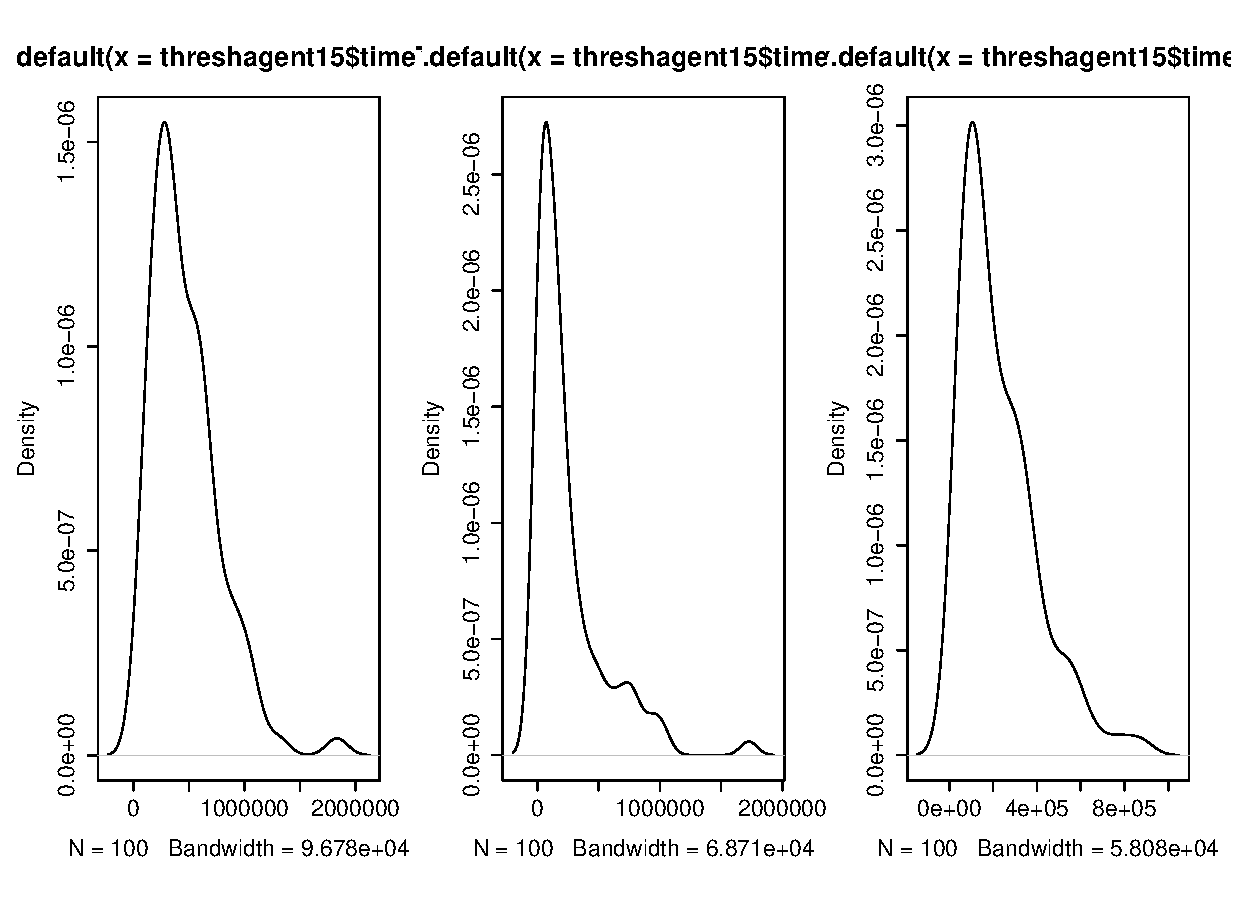
\includegraphics[width=0.7\textwidth]{densitythreshagent15}
    \caption{Density plots for run 8}
    \label{fig:densitythreshagent15}
\end{figure}

\begin{figure}[H]
    \centering
    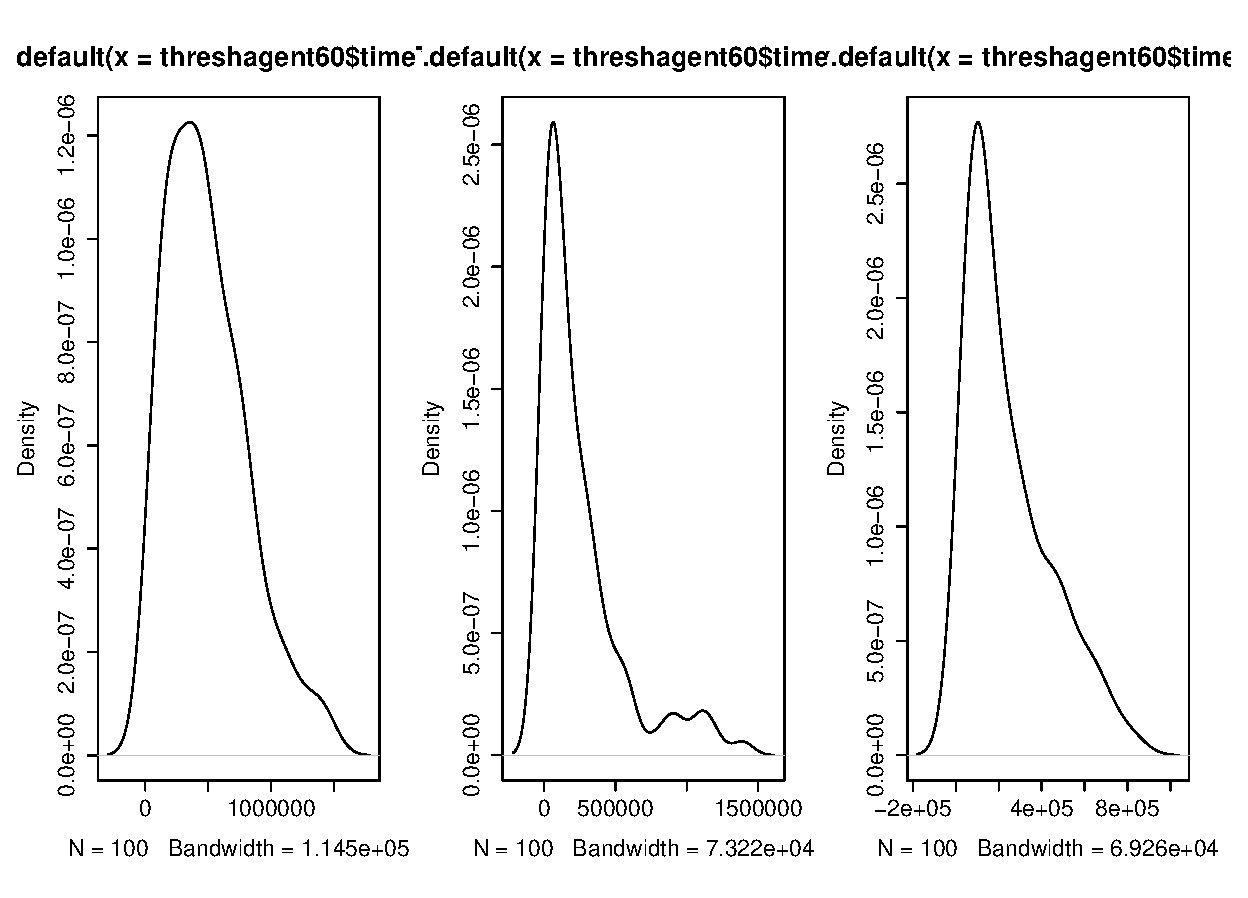
\includegraphics[width=0.7\textwidth]{densitythreshagent60}
    \caption{Density plots for run 9}
    \label{fig:densitythreshagent60}
\end{figure}

\begin{figure}[H]
    \centering
    \includegraphics[width=0.7\textwidth]{densitythreshagent120}
    \caption{Density plots for run 10}
    \label{fig:densitythreshagent120}
\end{figure}

\begin{figure}[H]
    \centering
    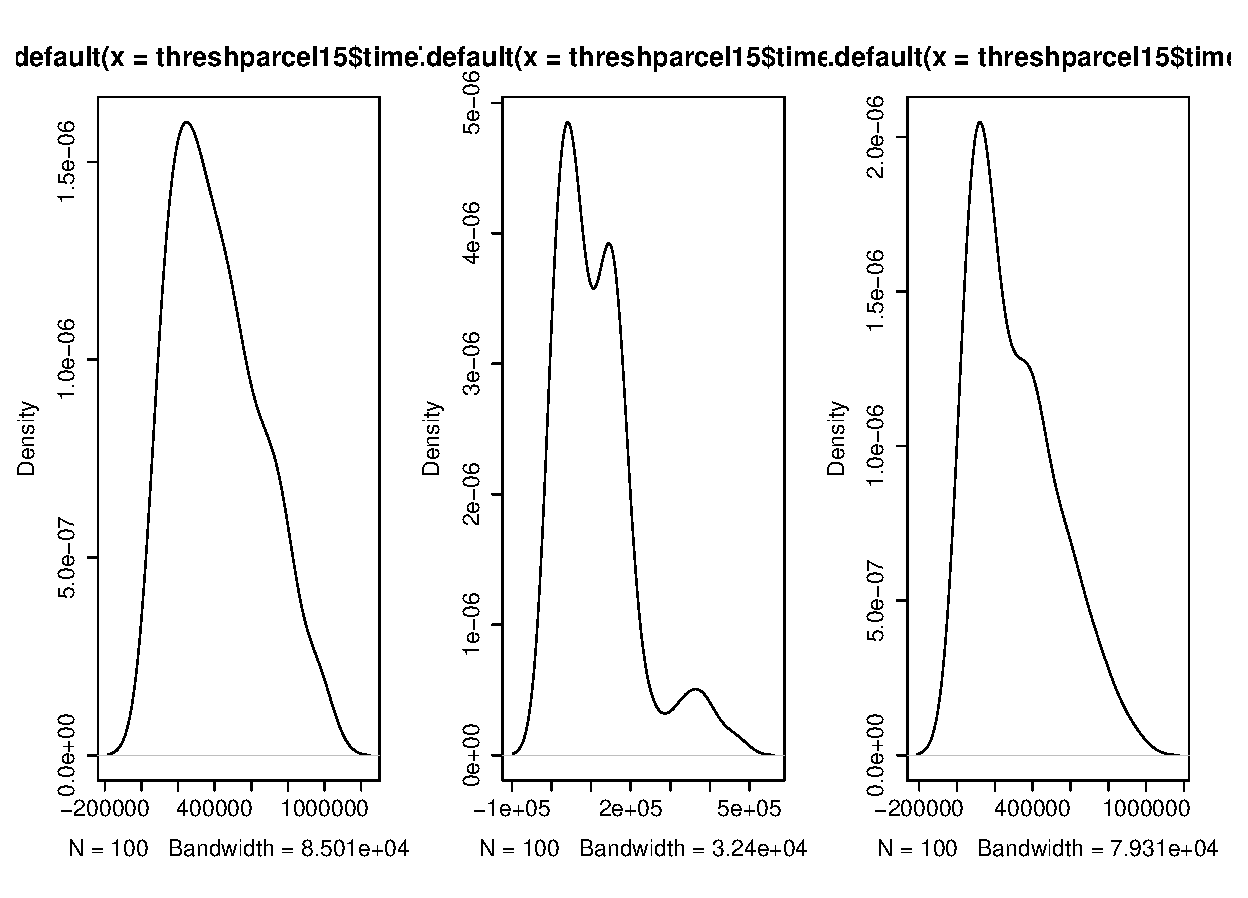
\includegraphics[width=0.7\textwidth]{densitythreshparcel15}
    \caption{Density plots for run 11}
    \label{fig:densitythreshparcel15}
\end{figure}

\begin{figure}[H]
    \centering
    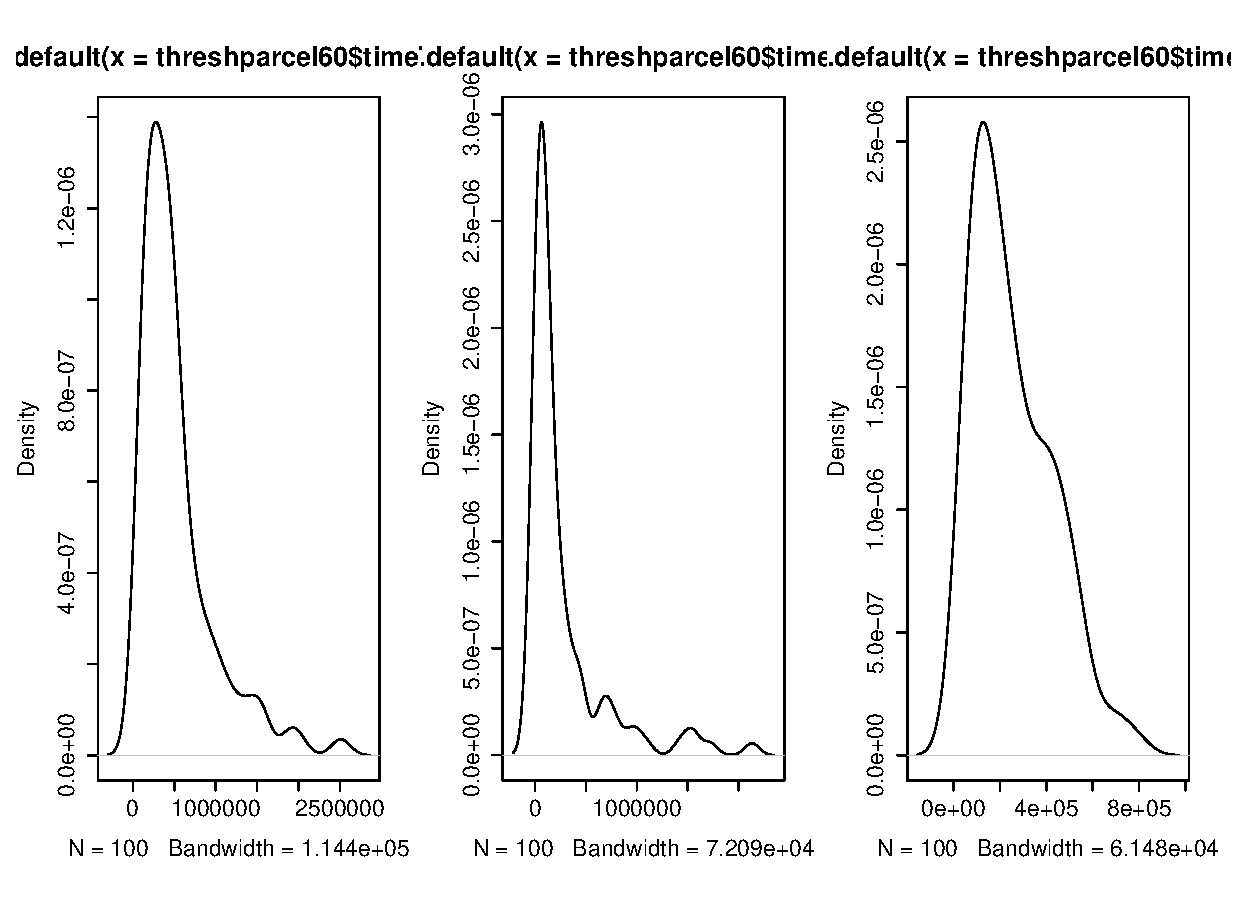
\includegraphics[width=0.7\textwidth]{densitythreshparcel60}
    \caption{Density plots for run 12}
    \label{fig:densitythreshparcel60}
\end{figure}

\begin{figure}[H]
    \centering
    \includegraphics[width=0.7\textwidth]{densitythreshparcel120}
    \caption{Density plots for run 13}
    \label{fig:densitythreshparcel120}
\end{figure}

\subsection{Analysis of the results}
First of all, we check whether we can assume that the parcel delivery times, pick-up times and times on route are respectively normally distributed for the reference model. Figure \ref{fig:refqq} depicts the relevant quantile plots. For each plot, we can see that there are clear deviations from the line, indicating that none of the samples are drawn from a normal distribution. This is supported by the respective p-values resulting from the Shapiro-Wilk test \cite{wiki:shapiro} of $7.743 \times 10^{-7}\%$, $9.514 \times 10^{-12} \%$ and $1.743 \times 10^{-4}\%$. Therefore, we will always use the median as the estimator for the expected value and use the Mann-Whitney U test \cite{wiki:mann-whitney} when testing for location shifts (i.e. difference in median), since the paired t-test assumes that the tested samples are both drawn from normally distributed populations \cite{wiki:ttest}, and we will always compare data from the runs to data from the reference model.

\begin{figure}[H]
    \centering
    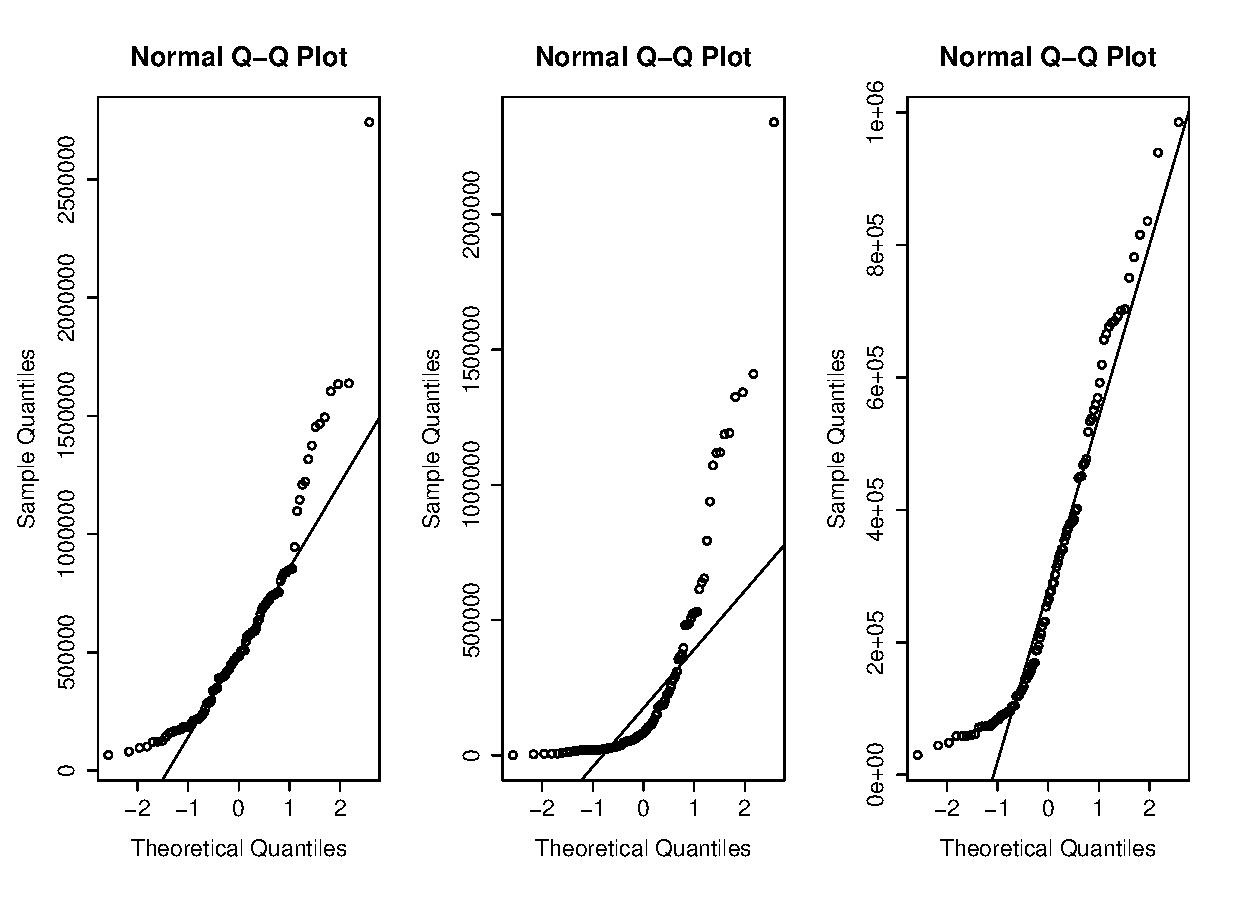
\includegraphics[width=0.7\textwidth]{refqq}
    \caption{Quantile plots for the reference model. The left plot is for parcel delivery times, the middle plot is for pick-up times and the right plot is for times on route.}
    \label{fig:refqq}
\end{figure}

\begin{table}[h]
    \begin{tabular}{llll}
         & Parcel delivery time           & Pick-up time                     & Time on route                  \\
        Run 1                                        & $\mu = 483787.5$               & $\mu = 83223$                    & $\mu = 263400$                 \\
        Run 2                                        & $\mu = 524937.5, p = 14.63\%$  & $\mu = 265544.5, p = 0.1165\% *$ & $\mu = 163400, p = 1.264\% *$  \\
        Run 3                                        & $\mu = 433897, p = 94.45\%$    & $\mu = 180801.5, p = 5.985\%$    & $\mu = 159900, p = 0.1032\% *$ \\
        Run 4                                        & $\mu = 583372, p = 26,57\%$    & $\mu = 237845, p = 0.4188\% *$   & $\mu = 149900, p = 0.2121\% *$ \\
        Run 5                                        & $\mu = 377882, p = 21,23\%$    & $\mu = 92671.5, p = 38,57\%$     & $\mu = 170600, p = 0.8966\% *$ \\
        Run 6                                        & $\mu = 489506, p = 93.28\%$    & $\mu = 152076, p = 22.55\%$      & $\mu = 211200, p = 19.57\%$    \\
        Run 7                                        & $\mu = 360977, p = 0.1237\% *$ & $\mu = 84867.5, p = 18.34\%$     & $\mu = 212100, p = 30.76\%$    \\
        Run 8                                        & $\mu = 394149, p = 9.588\%$    & $\mu = 139320, p = 33.08\%$      & $\mu = 174900, p = 1.18\% *$   \\
        Run 9                                        & $\mu = 459588, p = 19.96\%$    & $\mu = 139253, p = 37.91\%$      & $\mu = 176400, p = 2.752\% *$  \\
        Run 10                                       & $\mu = 394658, p = 16.3\%$     & $\mu = 143285.5, p = 19.62\%$    & $\mu = 193900, p = 3.124\% *$  \\
        Run 11                                       & $\mu = 370341, p = 1.231\% *$  & $\mu = 83706.5, p = 22.14\%$     & $\mu = 250600, p = 83.83\%$    \\
        Run 12                                       & $\mu = 403405.5, p = 12.7\%$   & $\mu = 110360, p = 64.86\%$      & $\mu = 208900, p = 20.78\%$    \\
        Run 13                                       & $\mu = 464860, p = 76.47\%$    & $\mu = 140984, p = 91.73\%$      & $\mu = 245400, p = 67.79\%$   
    \end{tabular}
    \caption{Results for each run. In every cell, the median and p-value from the Mann-Whitney U test are reported. P-values that indicate significance are marked with an asterisk (*). Run 1 does not report p-values since this run corresponds to the reference model.}
    \label{tbl:results}
\end{table}

Table \ref{tbl:results} reports for each run and dependent variable the median and the p-value resulting from the Mann-Whitney U test. Each test was run on a significance level of 5\%. The following observations can be made:
\begin{itemize}
    \item The models where the field strength of agents grows linearly with time seem to have consistently worse pick-up time and consistently better time on route (with significant effects observed for all three runs, namely 2, 3 and 4). This is plausible since agents will make way for other agents that are carrying a parcel with a high parcel waiting time instead of going to parcels that have yet to be picked up. It therefore seems that this method may be worth investigating if agent designers wish to reduce the time that agents are carrying parcels.
    \item Run 5 shows that having the field strength of parcels grow linearly with time, with a \emph{time-factor} of 15,000 milliseconds, seems to have a positive influence on the time on route. Furthermore, run 7, which has a \emph{time-factor} of 120,000 milliseconds, seems to have a significantly better parcel delivery time compared to reference. This seems to indicate that having the field strength of parcels linearly depend on the parcel waiting time may be worthwhile.
    \item Similarly to the first observation, having the agents increase their field strength when carrying a parcel that has reached a certain parcel waiting time seems to significantly reduce the time on route, as seen in runs 8, 9 and 10. The pick-up time is still consistently negatively influenced, but not enough to be significant. This method may also be worthwhile if agent designers wish to reduce the time that agents are carrying parcels.
    \item Run 11 shows that having parcels that have not yet been picked up and have reached a certain parcel waiting time of 15,000 milliseconds increase their field strength seems to have a significant positive influence on the parcel delivery time. This seems to indicate that this method of varying the gradient field strength of the parcels may be worth investigating.
\end{itemize}

It is not our ambition to claim that we have successfully provided an answer to the research questions. However, the above observations indicate that further investigation of models similar to the ones we have developed may be warranted.